\documentclass[tikz, border=1mm]{standalone}
\usepackage{tikz} 
\usetikzlibrary{arrows.meta}
\usepackage{pgfplots}

\begin{document}

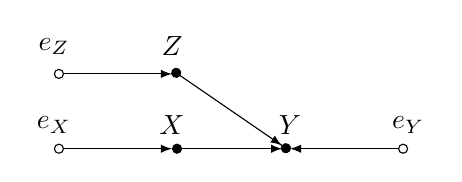
\begin{tikzpicture}

    % nodes (variables)
    \node at (-3,3) {$e_{Z}$};
    \node at (-1.5,3) {$Z$};
    \node at (-3,2) {$e_{X}$};
    \node at (-1.5,2) {$X$};
    \node at (0,2) {$Y$};
    \node at (1.5,2) {$e_{Y}$};
    
	% edges
    \draw[{Circle[open]}-{latex}](-3,2.65) to (-1.5,2.65); % e_{Z} -> Y
    \draw[{Circle}-{latex}{Circle}](-1.5,2.7) to (0,1.67); % Z -> Y
    \draw[{Circle[open]}-{latex}](-3,1.7) to (-1.5,1.7); % e_{X} -> Y
    \draw[{Circle}-{latex}](-1.5,1.7) to (-0.1,1.7); % X -> Y
    \draw[{Circle[open]}-{latex}](1.5,1.7) to (0,1.7); % e_{Y} -> Y    

\end{tikzpicture}

\end{document}
